\chapter{Introduction}


The rapid pace of global change poses a significant and ever-present threat to human prosperity. To facilitate the development of remediation technologies and enable effective mitigation strategies, we must make \textit{data-driven decisions}. However, the limitations posed by the lack of highly available, highly resolved data coupled together with the computational difficulties posed by direct simulation of physics \textit{at scale} severely constrains our ability to make the low uncertainty predictions needed to meaningfully address these challenges. The goal of this applied physics dissertation is to expand the boundary of what is possible in realm of sensing by leveraging machine learning in a \textit{principled way} to produce actionable insights. To that end, this work invokes three key case studies to demonstrate how machine learning can be used effectively to fill to enable


To that end, the guiding question of this work can be summarized succinctly as: \textit{How can we best utilize the measurements we have together with the physics we know to estimate the quantities we care about?}




- first we should discuss global change and the necessity for improved sensing and simulation
- justify the use of machine learning in order to fill the gaps where theory provides the motivation between what we measure and what we want to predict but no easily-represented physical relationship exists.
- this is a good place to bring in the
- we can then discuss the advent of physics-informed machine learning, and better, scientific machine learning to fill in the gaps and not be Snake Oil Salesmen (TM). In particular the role of numerical methods has not been subsumed by machine learning. At best these techniques are complementary and any performance claims need to be carefully benchmarked so as to not oversell the abilities of machine learning.
- Many of these emerging methods are promising but have seen little application to noisy, real-world data. One can only examine the Lorentz equations so much before transitioning to actual atmospheric dynamics
- We can do a paragraph on the specific areas we are trying to address: (1) using machine learning to establish the nonlinear relationship between measured spectra and constituent concentrations in water, (2) data-based techniques for evaluating the uncertainty of single sensor time series with application to low cost sensing, (3) physics based models for time series dynamics of Air Quality data (i.e. there will never be enough sensors on a low cost station to explain variability -- we would need a car presence sensor, etc... but we can model most of the dynamics and treat the rest as intermittent forcing), (3) how can we fuse sensing and simulation in order to infer the abundance of chemicals below detectable limits (in particular with application to indoor air chemistry).




\subsection{Global Change and the Need For Improved Sensing}

\subsection{Attention Towards Indoor Air Quality}

Humans spend approximately 90\% of their time indoors \cite{finewax_quantification_2021}. Consequently, the quality of indoor air has a dramatic effect on physical health, cognitive performance, and general well-being \cite{Krebs2021AirPC, Gao2021ShorttermAP, Carneiro2021TheEO, Ni2021AssociationsOP, Shehab2019EffectsOS}. At the beginning of the 20\textsuperscript{th} century, the debate about indoor air quality standards centered around quantifying the ideal ventilation rate for a variety of indoor spaces, ultimately leading to the ventilation rate procedure of ASHRAE standard 62. Engineers using this method compute the total outdoor ventilation rate by using the predefined rate-per-person and rate-per-area values for each desired space. Adjusting the ventilation rate is clearly effective for treating stale air and reducing so-called sick-building syndrome, but when dealing with contaminants and airborne pathogens, solely adjusting the ventilation rate falls short.

HVAC systems are typically designed to circulate air throughout a building, bringing in outside air, in order to achieve comfortable thermal conditions while consuming as little energy as possible \cite{memarzadeh_role_2012}. When assigned the secondary task of maintaining indoor air quality, ventilation operates by the same principles as a laboratory fume hood: airtightness and controlled airflow. To be effective, the ventilation system must move air along a short, unimpeded path toward the exhaust point while preventing unintended leakage \cite{ng_iaq_2015}. Despite these assumptions, most buildings are not airtight nor are they well-mixed \cite{emmerich_investigation_2005}. Further, the variable nature of indoor human interactions coupled with the plethora of possible room configurations introduces significant design challenges. For example, computational fluid dynamics simulations of the airflow in hospital rooms found that ``the most important contributing factor to contaminant transmission in enclosed and mechanically ventilated environment is the path between the contaminant source and the exhaust, not the air changes per hour" \cite{memarzadeh_role_2012}. This observation is widely confirmed across the literature with multiple studies indicating that air changes per hour (ACH) can be safely lowered without increasing concentrations of chemicals of concern above tolerable levels \cite{ng_IAQ_2015, lamping_air_nodate, li_evaluation_2014}. In concert with these findings, studies of the transmission of airborne pathogens suggest that “increasing the air change rate removes virus from the source room faster but also increases the rate of exposure in connected rooms. Therefore, slower air change rates reduce infectivity in connected rooms at shorter durations \cite{pease_investigation_2021}. 

As airborne transmission became the clear mechanism of SARS-CoV-2 spread, multiple studies confirmed the negative consequences of high air change rates. One study observed that when ACH was increased from 1.8 to 12, the time to peak virus concentration in connected rooms decreased from 30 minutes to 11 \cite{pease_investigation_2021}. A separate contact-tracing case study found that six students were infected by a teacher in a distant room, despite the use of high-efficiency particulate air filters throughout the building \cite{turakhia_ultrafast_2021}. Indeed, amidst observations of increased HVAC energy consumption by upwards of 128\% in one Chinese district, researchers still concluded that “HVAC systems may turn out to be the culprit of microbial contamination in enclosed spaces and deteriorate the environment due to inappropriate design and operation”  \cite{zheng_covid-19_2021}.

Filtration by means of in-room high-efficiency particle air (HEPA) and gas-phase filters suffer from the same limitations as discussed above. Namely, air filters only clean the air they come into contact with. This establishes a dichotomy between air quality goals and energy expenditure: pulling less outdoor air is more efficient, but pulling less air through filtration reduces efficacy \cite{lamping_air_nodate}. Often, the flow rates needed to have a positive effect are far less than the suggested ventilation rates offering opportunities for energy savings. This is the spirit of the alternative ASHRAE 62 IAQ procedure which seeks to attain acceptable indoor air quality by performance-based design criteria. One challenge of IAQP methods is one should predetermine contaminants of concern together with their acceptable levels in order to regulate building design \cite{zaatari_impact_2016}. Buildings contain significant sources of volatile chemical products such as cleaners, disinfectants, personal care products (PCPs), and paints whose use introduces a variety of potentially harmful compounds into the indoor \hbox{environment \cite{finewax_quantification_2021}}. The need to reduce energy use while treating  contaminants of concern and infectious microorganisms is the motivation for our response to this RFI. Improved characterization of the built environment together with \textit{active} air treatment technologies like ActivePure provides low-cost means to optimize building energy consumption without sacrificing the quality of our air.


HVAC system operating costs account for a significant portion of the total energy consumption in buildings, which themselves account for 40\% of the total energy consumption in the United \hbox{States \cite{ng_IAQ_2015}}. In the retail sector alone, ventilation accounts for 8.4\% of the total energy consumption and 27.8\% of the gas energy consumption \cite{zaatari_impact_2016}. It comes as no surprise, then, that the carbon footprint associated with those activities must decrease in the coming years in order to meet global decarbonization targets. 

%The growing body of pandemic case studies calls into question the long-held belief that increasing ventilation is the only and best way to control indoor pollution and reduce the spread of airborne pathogens \cite{ng_IAQ_2015, zaatari_impact_2016, pease_investigation_2021, zheng_covid-19_2021}. 

Furthermore, such proposals to focus on increased ventilation rates can only be realized through significant construction and renovation, and once completed, have a significant increase in running costs due to the energy required, preventing our most vulnerable communities from accessing clean air disproportionately \cite{lamping_air_nodate}. The federal government should first recognize that \textbf{any solution that involves even a minor increase in cost or carbon footprint is a non-starter for many decision-makers}.

The authors of this response hear this market feedback on a daily basis and are constantly on the lookout for behaviors and actions by these decision-makers that align with this mindset. Changing this mindset will be incredibly challenging, especially given that the majority of Americans believe the worst of the pandemic has passed. Instead, we have the option to accept this reality and work within its constraints to achieve the greatest good.  Fortunately, a \lq Clean First' \citep{enVerid, enVeridWhitePaper} approach would give the Federal Government the best chance of making improvements that will result in tangible results in better health and safety for all Americans.

While the passage of the Clean Air Act was a defining moment, and subsequent updates have been invaluable, the recent pandemic has unequivocally demonstrated the need for improved EPA testing and evaluation methodology that characterizes the various components of indoor air quality holistically. This is necessary for the critical evaluation and assessment of built-environment ventilation, filtration, and air-cleaning approaches. Furthermore, given the dual challenges of global pandemics and global change, the carbon footprint of various indoor air quality remediation strategies must be evaluated in order to optimize both indoor air quality and the carbon footprint. If we fail to consider both aspects, we risk inadvertently promoting an increase in health and economic disparities by failing to consider the very real fiscal cost associated with increased air changes. It is time to enable holistic optimization of both indoor air quality and energy (and carbon footprint) impacts.

The need for this dual optimization of indoor air quality and energy consumption goes beyond extreme events such as the COVID-19 pandemic. Without a doubt, the composition of the ambient environment has a significant impact on human health as well as general human physical and cognitive performance. We take this reality as a foundational premise in areas such as Chemical, Biological, Radiological, and Nuclear (CBRN) defense, but it appears to be all too easily overlooked when it comes to everyday occupational exposures that, when aggregated across society, may be far more significant. For example, society rarely, if ever, considers the impact of chemical emissions from personal care products, bleach, air fresheners, disinfectants, and even human excretions on indoor air quality. Each of these causes our buildings to contain a slew of volatile organic compounds \cite{finewax_quantification_2021}, as well as reactive halogen species from bleaches.


\begin{table}[h!]
  \centering
  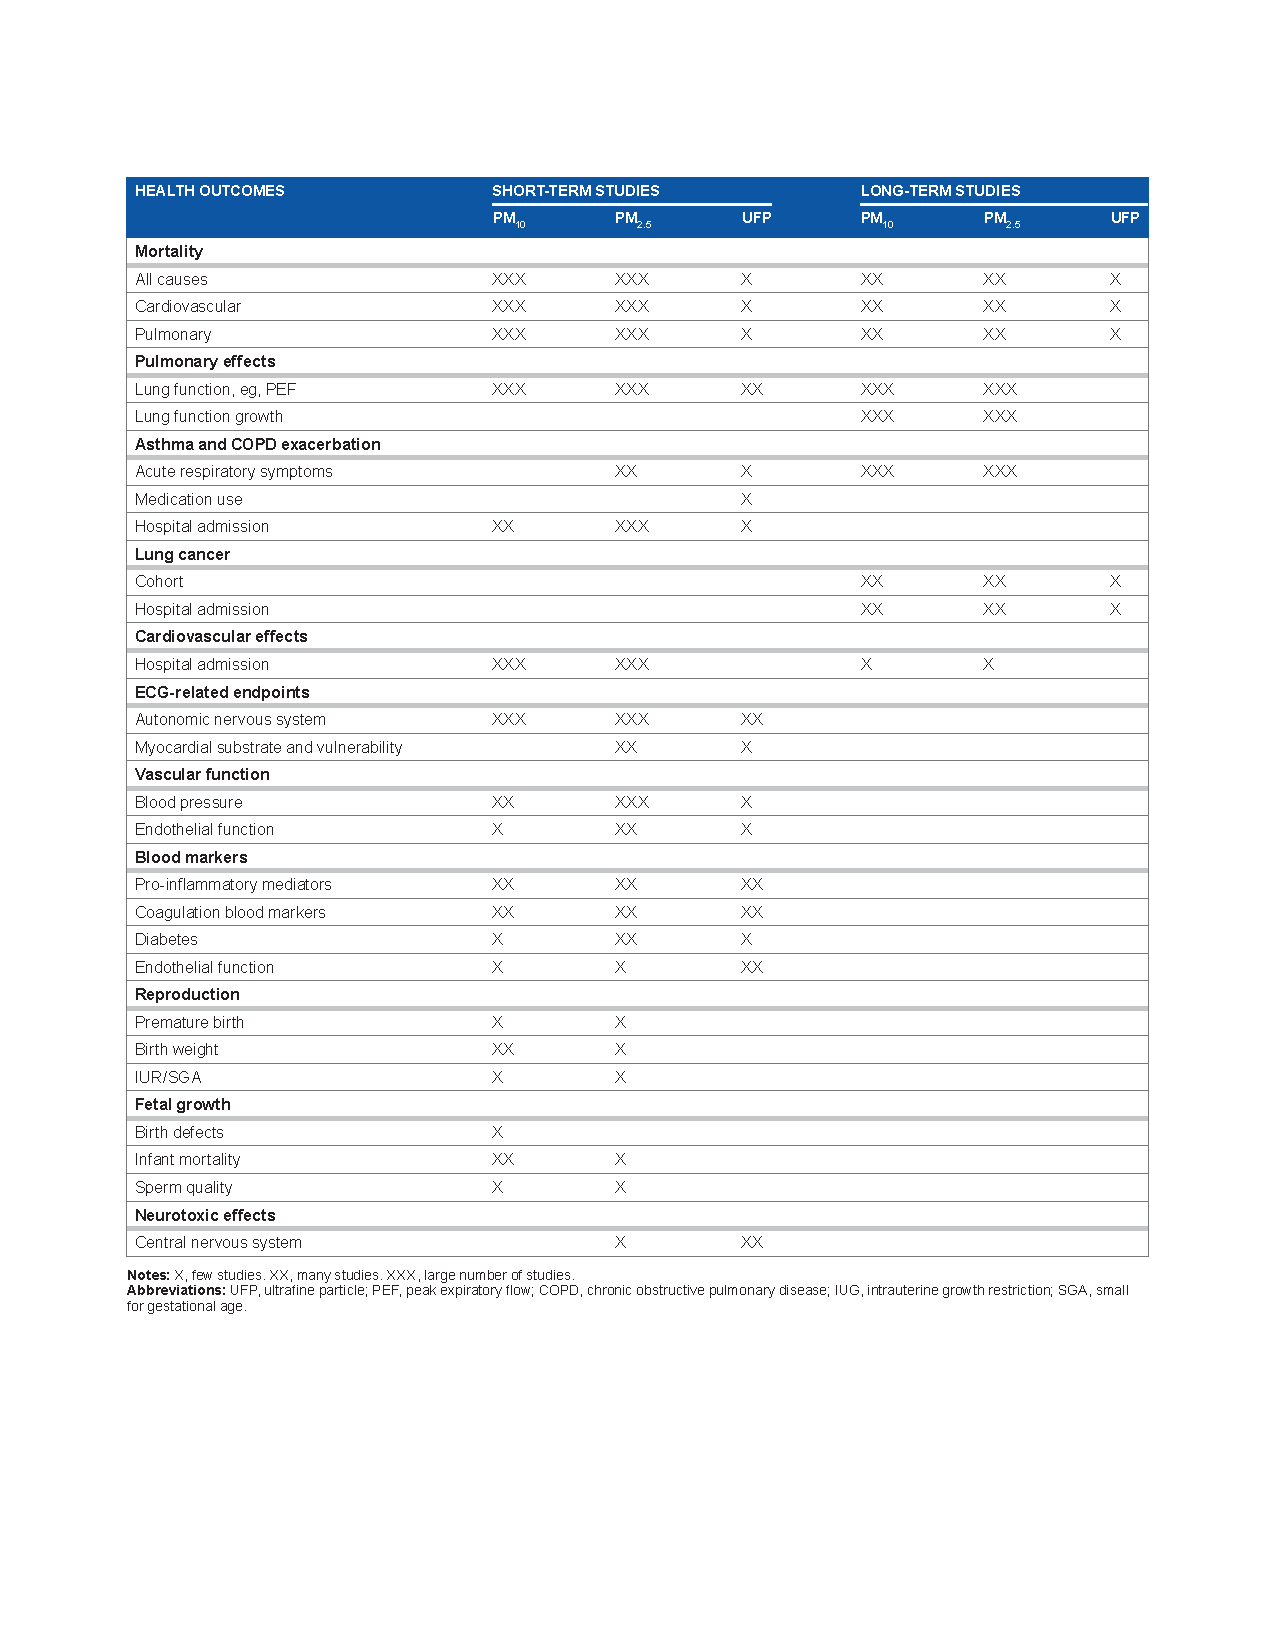
\includegraphics[width=\textwidth]{introduction/HealthEffectsParticulates.pdf}
	\caption{Tabular literature review of particulate matter and health outcomes related to PM$_{10}$, PM$_{2.5}$, and ultrafine particulates (UFPs) exposure (based on the literature review of \cite{Lary:2015}).}
	\label{Table.HealthEffectsParticulates}
\end{table}


Even after a significant initial indoor exposure event may have passed, the health impact associated with prior significant and persistent exposure events may well contribute to long-term health quality. For example, chemical disinfectants such as hypochlorite bleach, have been linked to respiratory ailments and have been observed to produce harmful byproducts such as chloroform, carbon tetrachloride, and N-chloroaldimines, which can take up to 3 hours to be ventilated away after the use the bleach  \cite{finewax_quantification_2021, odabasi_halogenated_2008}. EPA testing needs to consider a maximal set of components, not a minimal set of only a few criterion pollutants, and we know that COVID-19 was spread through inadequately treated indoor air.  It is therefore critical that the EPA testing for indoor air quality in the built environment is rigorous, comprehensively characterizing all aspects of indoor air quality, going beyond the outdoor National Ambient Air Quality Standards (NAAQS). It is clearly time for a strategy that goes well beyond just six criteria air pollutants.

For example, some work in this area identifies a short list of species based on a metric widely used by the World Health Organization, the Disability Adjusted Life Years (DALY) indicator (means \lq loss of life corrected by disability') \cite{Juginovi:2021, Lehtomki:2018}. The DALY indicator is widely used to assess the disease burden on the population and identify disease causes. According to the World Health Organization (WHO), ambient air pollution causes 4.2 million premature deaths worldwide each year. In comparison, the total number of global confirmed COVID-19 deaths in 2020 was 1.9 million, and 3.6 million in 2021. Even at the height of the COVID pandemic, deaths from poor air quality outnumbered those from COVID-19. The quality of outdoor ambient air, in turn, influences the quality of indoor air. In areas where outdoor air quality is already poor, increasing ventilation inevitably introduces pollutants indoors, even when filtration is employed \cite{srikrishna_long-term_2022}.

While death is unquestionably the most severe consequence of pollution, it is far from the only one. The biological wear and tear caused by poor air quality (allostatic load) have been shown to degrade cognitive and physical performance, as well as a variety of human health outcomes \cite{Krebs2021AirPC, Gao2021ShorttermAP, Carneiro2021TheEO, Ni2021AssociationsOP, Shehab2019EffectsOS}.


To illustrate, even among the indoor particulates with representatives among the criterion pollutants (PM$_{2.5}$ and PM$_{10}$), the ultra-fine particulate matter, with a size of less than 0.1 $\mu$m,  are not included among the criterion pollutants, yet  are actually some of the most dangerous to human health \cite{Ehsanifar:2021, Ehsani:2022, Ehsanifar:2022b, Zhang:2019}. The ultra-fine size fraction penetrates most deeply into the lungs, and can readily get into the bloodstream, and even into the brain across the blood-brain barrier. On this point, it is worth noting that there is a substantial increase in Alzheimer's which is associated with inflammation in the brain \cite{Urrutia:2021}. Ultra-fine particulates are known to be associated with brain \hbox{inflammation \cite{Rhew:2021}}. Further, at the other end of the size spectrum, the larger size range above \hbox{10 $\mu$m} is also currently excluded from EPA testing. This larger size range includes some airborne molds and pollens associated with some of the significant allergies prevalent across society \cite{DAmato:2020}. A similar issue is present with volatile organic compounds (VOCs), and the inappropriate lumping of very different types of organic compounds.

It is not just health outcomes, such as those listed in Table~\ref{Table.HealthEffectsParticulates}, that are associated with poor air quality. Numerous studies have demonstrated that poor air quality diminishes both human cognitive and physical performance \cite{Krebs2021AirPC, Gao2021ShorttermAP, Carneiro2021TheEO, Ni2021AssociationsOP, Shehab2019EffectsOS}. Degraded cognitive performance has a significant impact on society, ranging from poor learning outcomes in schools to impaired decision-making performance and productivity at work. As a result, the ability to adequately and comprehensively quantify the performance of indoor air quality remediation systems is critical for guiding appropriate, science-based threat mitigation strategies. If HVAC control is driven by an incomplete subset of metrics/contaminants of concern, buildings will clearly fail to adapt to unexpected threats. For instance, CO$_2$ is frequently used as a control metric because it acts as a tracer gas to control the ventilation rate per person by controlling the indoor/outdoor differential. However, using CO$_2$ along with other metrics is beneficial. For example, five studies found that CO$_2$ control alone cannot control for pollutants generated outdoors or indoors independent of human activity \cite{zaatari_impact_2016}. More recently, one COVID-19 case study discovered that the rapid spread of the disease through a nursing home ward was most likely caused by decreased ventilation by a CO$_2$ demand control ventilation system optimized solely for decreased energy-demand \cite{lamping_air_nodate}.




\subsection{Physics Informed Machine Learning}

\subsection{Dissertation Overview}





Much of the current machine learning landscape is dominated by highly abstract problems like image recognition, language prediction

In particular, this work focuses on three key areas

we should not throw the baby out with the bath water. Nor should we attempt to reinvent the wheel... we can use machine learning to \textit{fill in the gaps} where our current theory can not easily provide a direct link between the data we have and the target we wish to model but a relationship is easily justified on physical grounds. Further, we can use our knowledge of physical laws to impose strong constraints on the space of available models that may significantly improve the capability of machine learning models to extrapolate beyond the boundaries of their training data sets. 

make the point that for physical theories are typically only amenable to analytic techniques when sufficiently constrained to domains with high symmetry or where nonlinear interactions can be controlled so that linear effects dominate over bounded of higher order effects (re: perturbation theory). For common real world scenarios where edges are sharp, functions aren't smooth, and approximating assumptions can not be readily applied, we typically must resort to numerical methods which seek to solve the dynamical laws on computational domains with well posed boundary and initial conditions.

In the first proposed project, we will apply machine learning techniques to provide a sensor calibration where theory suggests


To that end, this work focuses on improving sensing capabilities in three key domains: water quality, outdoor air quality, and indoor air quality.





physical sensing and physics-informed machine learning. The world we inhabit is undergoing rapid and transformative changes, with pressing environmental challenges demanding innovative solutions. At the heart of this quest lies the critical need for a deeper understanding of our complex environmental systems, coupled with the ability to derive actionable insights from the wealth of data at our disposal. This dissertation represents my contribution to addressing these challenges by bridging the gap between the physical world and advanced data-driven methodologies. Through the fusion of physical sensing technologies and machine learning, my research endeavors to unlock profound insights into environmental phenomena, ultimately facilitating informed decisions and sustainable practices in an ever-changing world.



This goal is pursued by applying physics informed approaches together with a suite of sensing and computational technologies, implementing the reusable paradigm of software defined sensors, i.e. physical sensing elements wrapped in a software layer. This software layer can serve a variety of purposes such as calibration and the provision of enhanced or derived data products. It is part of a broader effort in the MINTS-AI laboratory at the University of Texas at Dallas. Where MINTS-AI is an acronym, Multi-Scale Multi-Use Integrated Intelligent Interactive Sensing in Service of Society for Actionable Insights.

Comprehensive environmental sensing is a timely and beneficial endeavor for a variety of reasons. The growing awareness of major environmental issues such as climate change, pollution, and habitat loss necessitates effective environmental monitoring and management. Comprehensive environmental sensing can provide real-time data on air and water quality, weather patterns, and other environmental factors, assisting in the identification and resolution of environmental issues. This assists in the development and implementation of policies and strategies aimed at reducing environmental impact and increasing sustainability. Given that, for instance, air quality can have significant effects on human health, this has particular societal value.

Comprehensive sensing of the environment can improve decision-making. The real-time and accurate data provided by environmental sensors can aid in informed decision-making regarding various aspects such as traffic management, industrial regulation, and crop planning. For instance, data on air quality can be used to inform decisions about reducing pollution levels, while data on weather patterns can help farmers to plan their crops and reduce water usage. Comprehensive sensing of the environment can be instrumental in emergency response. Real-time data on weather patterns, air quality, water levels and resources, and seismic activity can help emergency responders to prepare for and respond to natural disasters such as hurricanes, floods, and earthquakes. The quick and accurate information can enable effective and timely response, potentially saving lives and reducing the impact of the disaster.

Many advances in technology have enabled the creation of comprehensive sensing systems that can monitor and analyze data from various sensors and devices in real-time. In this thesis we use a range of technologies including autonomous robotic teams [@Dunbabin2012; @Rubenstein2014; @Chen2017], hyperspectral imaging [@Plaza2009; @Li2018; @Zhu2017], mesh networks utilizing the Internet of Things (IoT) [@Gubbi2013; @Atzori2010; @Al-Fuqaha2015], machine learning (ML) [@Goodfellow2016; @LeCun2015; @Jordan2015], edge computing, high-performance computing,  wearable sensors and modern high-performance dynamic programming languages such as Julia [@Bezanson2017] designed for numerical and scientific computing. These technologies have facilitated the collection and processing of large amounts of data from multiple sources, resulting in more accurate and comprehensive environmental monitoring.



Today, the most well known application of machine learning techniques


%% \section{Completed Work}

%% \subsection{An Autonomous Robotic Team}
%% \subsection{A Distributed Network of Low-Cost Air Quality Monitors}

%% \section{Proposed Work}

%% \subsection{Robot Team}
%% \subsection{Air Quality Network}
%% \subsection{HEART Chamber}
